\documentclass[12pt,letterpaper]{article}
\usepackage{fullpage}
\usepackage[top=2cm, bottom=4.5cm, left=2.5cm, right=2.5cm]{geometry}
\usepackage{amsmath,amsthm,amsfonts,amssymb,amscd}
\usepackage{lastpage}
\usepackage{enumerate}
\usepackage{fancyhdr}
\usepackage{mathrsfs}
\usepackage{xcolor}
\usepackage{graphicx}
\usepackage{listings}
\usepackage{hyperref}

\hypersetup{%
  colorlinks=true,
  linkcolor=black,
  linkbordercolor={0 0 1}
}
 
\renewcommand\lstlistingname{Algorithm}
\renewcommand\lstlistlistingname{Algorithms}
\def\lstlistingautorefname{Alg.}

\lstdefinestyle{Python}{
    language        = Python,
    frame           = lines, 
    basicstyle      = \footnotesize,
    keywordstyle    = \color{blue},
    stringstyle     = \color{green},
    commentstyle    = \color{red}\ttfamily
}

\setlength{\parindent}{0.0in}
\setlength{\parskip}{0.05in}

% Edit these as appropriate
\newcommand\course{EECE 7047 Dynamic Optimization }
\newcommand\hwnumber{1}                  % <-- homework number
\newcommand\NetIDa{}           % <-- NetID of person #1
\newcommand\NetIDb{}           % <-- NetID of person #2 (Comment this line out for problem sets)

\pagestyle{fancyplain}
\headheight 35pt
\lhead{\NetIDa}
\lhead{\NetIDa\\\NetIDb}                 % <-- Comment this line out for problem sets (make sure you are person #1)
\chead{\textbf{\Large Exam \hwnumber}}
\rhead{\course \\ \today}
\lfoot{}
\cfoot{}
\rfoot{\small\thepage}
\headsep 1.5em

\begin{document}

Notes: 

Code for all answers using indirect shooting is written such that ALL state variables are "guesses", including those bounded by $\phi$. Those values which are known (through $\phi$ or through a derived solution, perhaps $\lambda_x$) are then set directly to be the guess made, and added as an additional part of the error vector.

In solutions, only values which are truly unknown (and have no constraint) will be marked as unknown. 

All analytically derived optimality conditions are will be attached and marked.

In all direct solutions, theta is kept track of in state so that it may be plotted, however, it is not used. 

\section*{Problem 1}

Problem 1 is answered by \path{problem1.m}, which depends on \path{dynamics1.m}, \path{error1_backwards.m}, and \path{error1_forwards.m}. 

The formulas derived analytically are attached. In the end, we find at $t_0$:

\begin{equation}
\begin{aligned}
\label{eq:2}
x(t_0) &= 0 \\
y(t_0) &= 2 \\
\lambda_x(t_0) &= ? \\
\lambda_y(t_0) &= ? 
\end{aligned}
\end{equation}

And at $t_f$:

\begin{equation}
\begin{aligned}
\label{eq:2}
x(t_f) &= 5 \\
y(t_f) &= ? \\
\lambda_x(t_f) &= \frac{1}{e^(-y(t_f)^2)} \\
\lambda_y(t_f) &= ? 
\end{aligned}
\end{equation}

Leaving the final values to solve for as $t_f$, $y(t_f)$, $\lambda_y(t_f)$, $\lambda_x(t_0)$ and $\lambda_y(t_0)$.

After running both forward and backward shooting methods, the solution is shown in Figure \ref{fig:prob1indirect}.

\clearpage


\begin{figure}[!h]
\centering
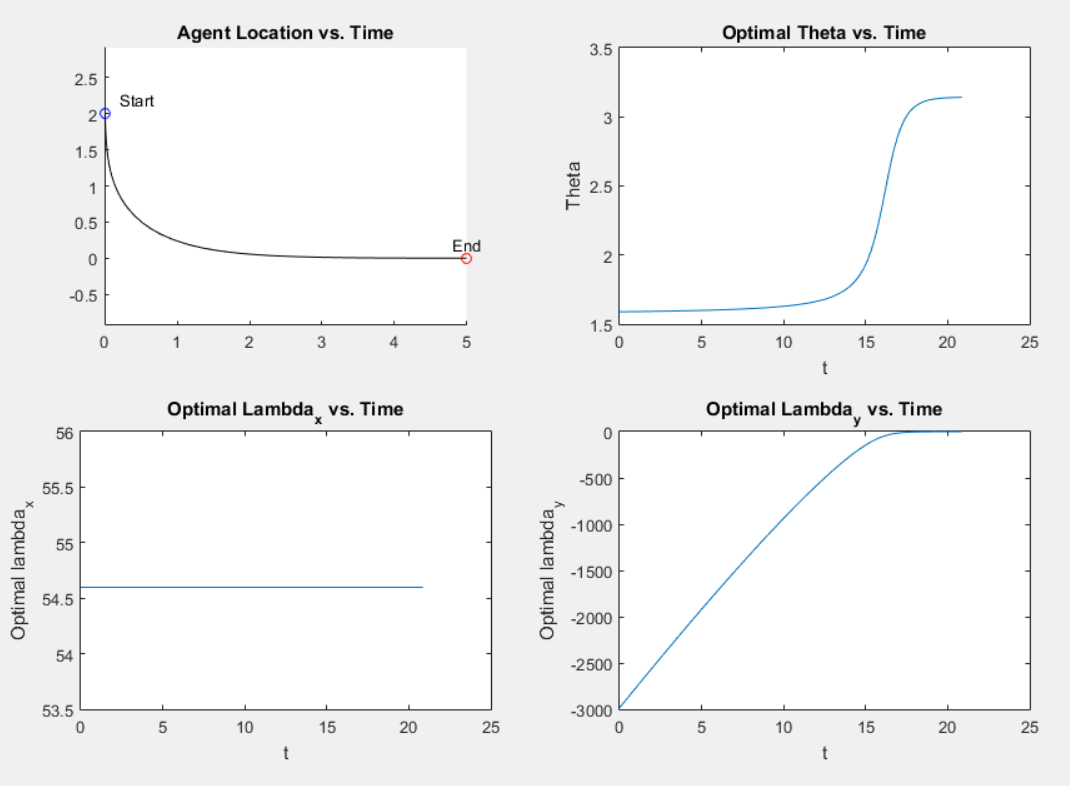
\includegraphics[width=5in]{prob1indirect.png}
\caption{Problem 1 Solved Indirectly}
\label{fig:prob1indirect}
\end{figure}

Figure \ref{fig:prob1indirect} shows a kind of "bang-bang" controller that has been smoothed out, which makes sense considering that a similar problem was done in class, without the exponential terms, which resulted in a pure "bang-bang" controller. 

Using indirect forward or backward shooting yielded an identical result. If the graph showing agent position is zoomed in on, it results in Figure \ref{fig:prob1zoom}.


\begin{figure}[!h]
\centering
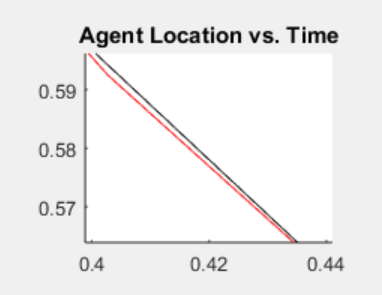
\includegraphics[width=3in]{prob1zoom.png}
\caption{Problem 1 Agent Position Expanded}
\label{fig:prob1zoom}
\end{figure}

Figure \ref{fig:prob1zoom} shows that the forward (red) and backward (black) solutions are essentially identical.

Problem 1 was also attempted via direct shooting in the file \path{problem1Direct.m}, which depends on \path{direct1Utility.m}, \path{direct1Dynamics.m}, and \path{direct1Constraint.m}. Because we the general form of the control and the derivatives of the adjoint variables have been derived, we can make an educated guess for $\theta$. The guess for the form was as follows:

\begin{equation}
\begin{aligned}
\label{eq:2}
\lambda_x &= c_1 \\
\lambda_y &= c_2*t^2 + c_3*t + c_4  \\
cos(\theta) &= -\lambda_x / \sqrt{\lambda_x^2 + \lambda_y^2} \\
sin(\theta) &= -\lambda_y / \sqrt{\lambda_x^2 + \lambda_y^2}
\end{aligned}
\end{equation}

These formulas were then used to calculate the dynamics. Unfortunately, using these dynamics resulted in an imperfect result. We know the general forms of the costate variables from above, however, it was difficult to find an exact form that would yield the same result as above. The final result is shown in Figure \ref{fig:prob1direct}.

\begin{figure}[!h]
\centering
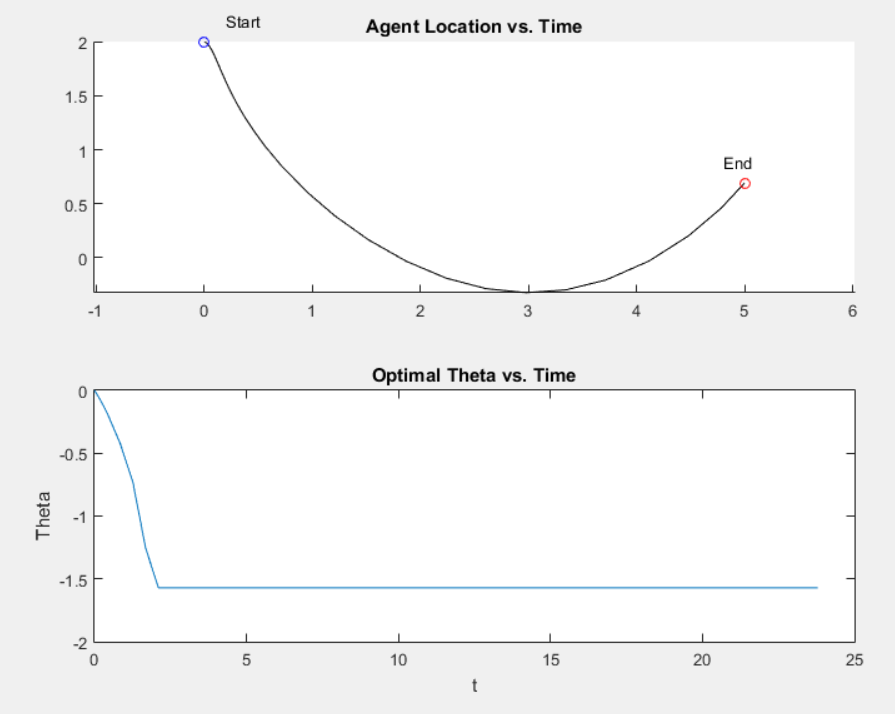
\includegraphics[width=5in]{prob1direct.png}
\caption{Problem 1 Solved Directly}
\label{fig:prob1direct}
\end{figure}

As can be seen in Figure \ref{fig:prob1direct}, the general form of the solution was correct, however, it was not quite optimal. Additionally, there were difficulties in obtaining $\theta$. Because it is not computed directly, we must take the inverse sine or cosine of the above equations, which results in imaginary numbers and the messy theta. In all, the indirect methods performed much better on this problem.

It was found that both backwards and forwards shooting worked for this problem. Using direct shooting yielded mixed results, likely due to the strange shape of theta. Other direct dynamics were attempted but were unsuccessful. Regardless, it is also inconvenient that theta is unable to be recovered, though using dynamics in terms of lambdas yielded the best final results.





\section*{Problem 2}

Problem 2 is answered by \path{problem2.m}, which depends on \path{dynamics2.m}, and \path{error2_backwards.m}. 

The formulas derived analytically are attached. In the end, we find at $t_0$:

\begin{equation}
\begin{aligned}
\label{eq:2}
x(t_0) &= 0 \\
y(t_0) &= 0 \\
v_x(t_0) &= 0 \\
v_y(t_0) &= 0 \\
\lambda_x(t_0) &= 0 \\
\lambda_y(t_0) &= ? \\
\lambda_{vx}(t_0) &= 1 \\
\lambda_{vy}(t_0) &= ?*t + ? 
\end{aligned}
\end{equation}

And at $t_f$:

\begin{equation}
\begin{aligned}
\label{eq:2}
x(t_f) &= ? \\
y(t_f) &= 5 \\
v_x(t_f) &= 0 \\
v_y(t_f) &= 0 \\
\lambda_(x)(t_f) &= 0\\
\lambda_{y}(t_f) &= ? \\ 
\lambda_(vx)(t_f) &= 1 \\
\lambda_{vy}(t_f) &= ?*t + ? 
\end{aligned}
\end{equation}

Leaving the final values to solve for as $t_f$, $x(t_f)$, $\lambda_y(t_f)$, $\lambda_{vy}(t_f)$, $\lambda_y(t_0)$, and $\lambda_{vy}(t_0)$.

After performing backward shooting, the solution is shown in Figure \ref{fig:prob2indirect}.


\clearpage


\begin{figure}[!h]
\centering
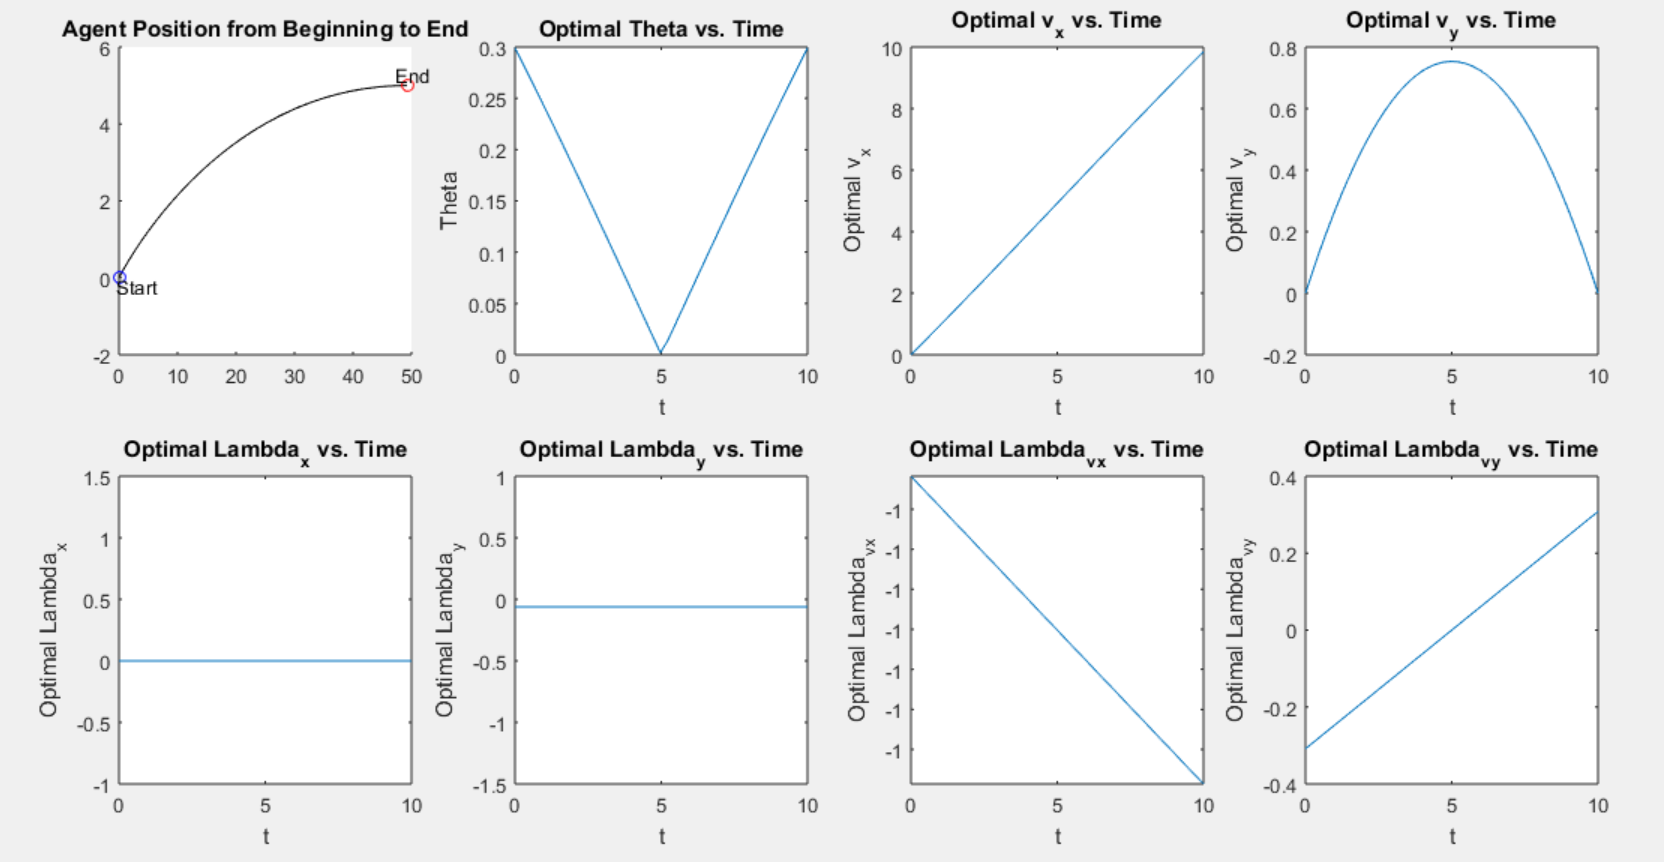
\includegraphics[width=6in]{prob2indirect.png}
\caption{Problem 2 Solved Indirectly}
\label{fig:prob2indirect}
\end{figure}

Problem 2 was also attempted using a direct solution in the file \path{problem2Direct.m}, which depends on \path{directUtility.m}, \path{directDynamics.m}, and \path{directConstraint.m}. Like Problem 1, we can guess the general shape of theta using the lambdas as derived: 

\begin{equation}
\begin{aligned}
\label{eq:2}
\lambda_{vx} &= -1 \\
\lambda_{vy} &= c_1*t^2 + c_2*t + c_3  \\
cos(\theta) &= -\lambda_{vx} / \sqrt{\lambda_{vx}^2 + \lambda_{vy}^2} \\
sin(\theta) &= -\lambda_{vy} / \sqrt{\lambda_{vx}^2 + \lambda_{vy}^2}
\end{aligned}
\end{equation}

This time, the same solution found via indirect shooting was found, as shown in Figure \ref{fig:prob2direct}.


\clearpage



\begin{figure}[!h]
\centering
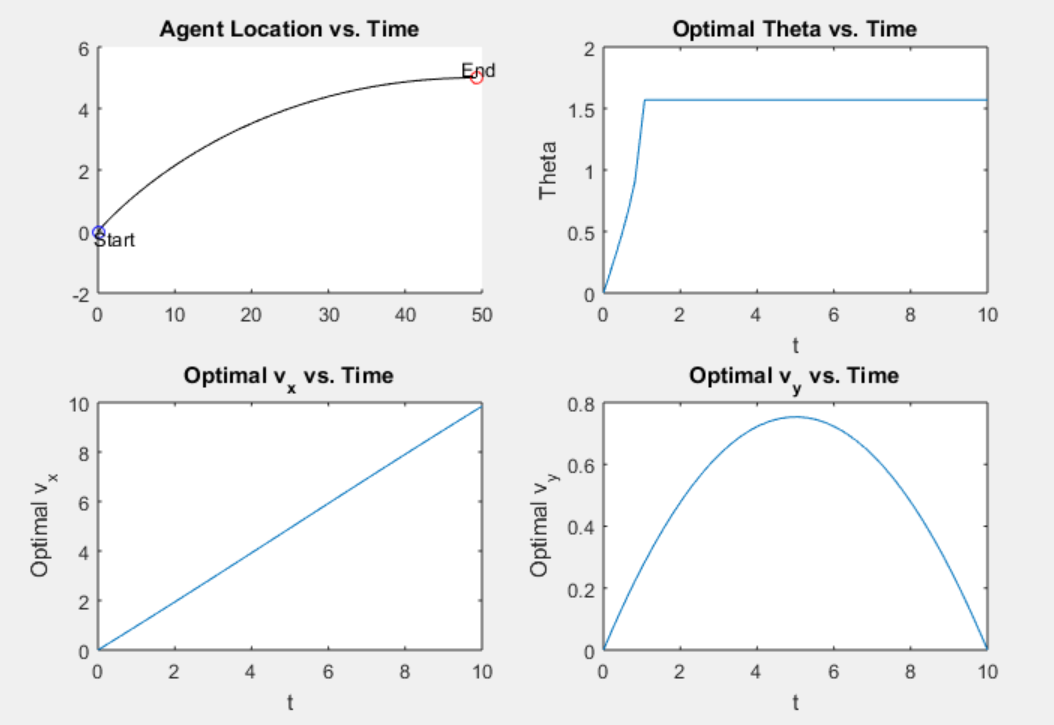
\includegraphics[width=4in]{prob2direct.png}
\caption{Problem 2 Solved Directly}
\label{fig:prob2direct}
\end{figure}

As can be seen in Figure \ref{fig:prob2direct}, the solution found was the same as the solution found with indirect shooting. Again, there were issues with actually finding $\theta$ as in Problem 1. It can be seen that $v_x$ and $v_y$ also match that of the indirect solution.


Problem 2 was able to be solved via both direct and indirect shooting, likely because theta ultimately takes a relatively simple shape (in comparison to problem 1). The "V" shape is much easier to recreate with custom dynamics. It is also inconvenient that theta is unable to be recovered, though using dynamics in terms of lambdas yielded the best final results.






\section*{Problem 3}

Problem 3 is answered by \path{problem3.m}, which depends on \path{dynamics3.m}, and \path{error3_backwards.m}.

The formulas derived analytically are attached. In the end, we find at $t_0$:

\begin{equation}
\begin{aligned}
\label{eq:2}
x_A(t_0) &= 0 \\
y_A(t_0) &= 10 \\
x_D(t_0) &= 5 \\
y_D(t_0) &= 0 \\
x_T(t_0) &= 0 \\
y_T(t_0) &= 0 \\
\lambda_{xA}(t_0) &= ? \\
\lambda_{yA}(t_0) &= ? \\
\lambda_{xD}(t_0) &= ? \\
\lambda_{yD}(t_0) &= ? \\
\lambda_{xT}(t_0) &= ? \\
\lambda_{yT}(t_0) &= ? \\
\end{aligned}
\end{equation}

And at $t_f$:

\begin{equation}
\begin{aligned}
\label{eq:2}
x_A(t_f) &= ? \\
y_A(t_f) &= ? \\
x_D(t_f) &= ? \\
y_D(t_f) &= ? \\
x_T(t_f) &= ? \\
y_T(t_f) &= ? \\
\phi(n) &= \sqrt{ (x_D(t_f) - x_A(t_f))^2 + (y_D(t_f) - y_A(t_f))^2 } \\
\Phi &= -\sqrt{ (x_T(t_f) - x_A(t_f))^2 + (y_T(t_f) - y_A(t_f))^2 } = 1 \\
\lambda_{xA}(t_f) &= \frac{x_A(t_f) - x_T(t_f)}{\Phi} + \nu*\frac{x_A(t_f) - x_D(t_f)}{\phi(n)}\\
\lambda_{yA}(t_f) &= \frac{y_A(t_f) - y_T(t_f)}{\Phi} + \nu*\frac{y_A(t_f) - y_D(t_f)}{\phi(n)} \\
\lambda_{xD}(t_f) &= \nu*\frac{x_D(t_f) - x_A(t_f)}{\phi(n)} \\
\lambda_{yD}(t_f) &= \nu*\frac{y_D(t_f) - y_A(t_f)}{\phi(n)} \\
\lambda_{xT}(t_f) &= \frac{x_T(t_f) - x_A(t_f)}{\Phi} \\
\lambda_{yT}(t_f) &= \frac{y_T(t_f) - y_A(t_f)}{\Phi} 
\end{aligned}
\end{equation}

Leaving the final values to solve for as all costate variables at $t_0$ and final positions for all agents. Costate variables at $t_f$ are bounded by the equations shown. 

Problem 3 was truly an odyssey to solve. Initially, replacing attacker dynamics with a new angle, $\theta_A$, was attempted. The entire problem was solved (the work will be attached), however, the answer looked strange as the agents all simply traveled in lines. In this answer, the defender traveled straight down, the attacker straight down, and the defender intercepted. It was believed that replacing the attacker dynamics with a new angle would only hold up if the derivatives were kept correct (e.g. what is $\frac{d\Lambda_{xA}}{dx_A} = \frac{dcos(\theta_A)}{dx_A}$, does this equal 0?). 

Keeping the attacker dynamics meant finding massive derivatives for costate dynamics and terminal adjoint conditions. These equations were found using wolframalpha and tweaked over sleepless nights while on Spring Break.

Eventually, the solution in Figure \ref{fig:prob3indirect} was found.

\begin{figure}[!h]
\centering
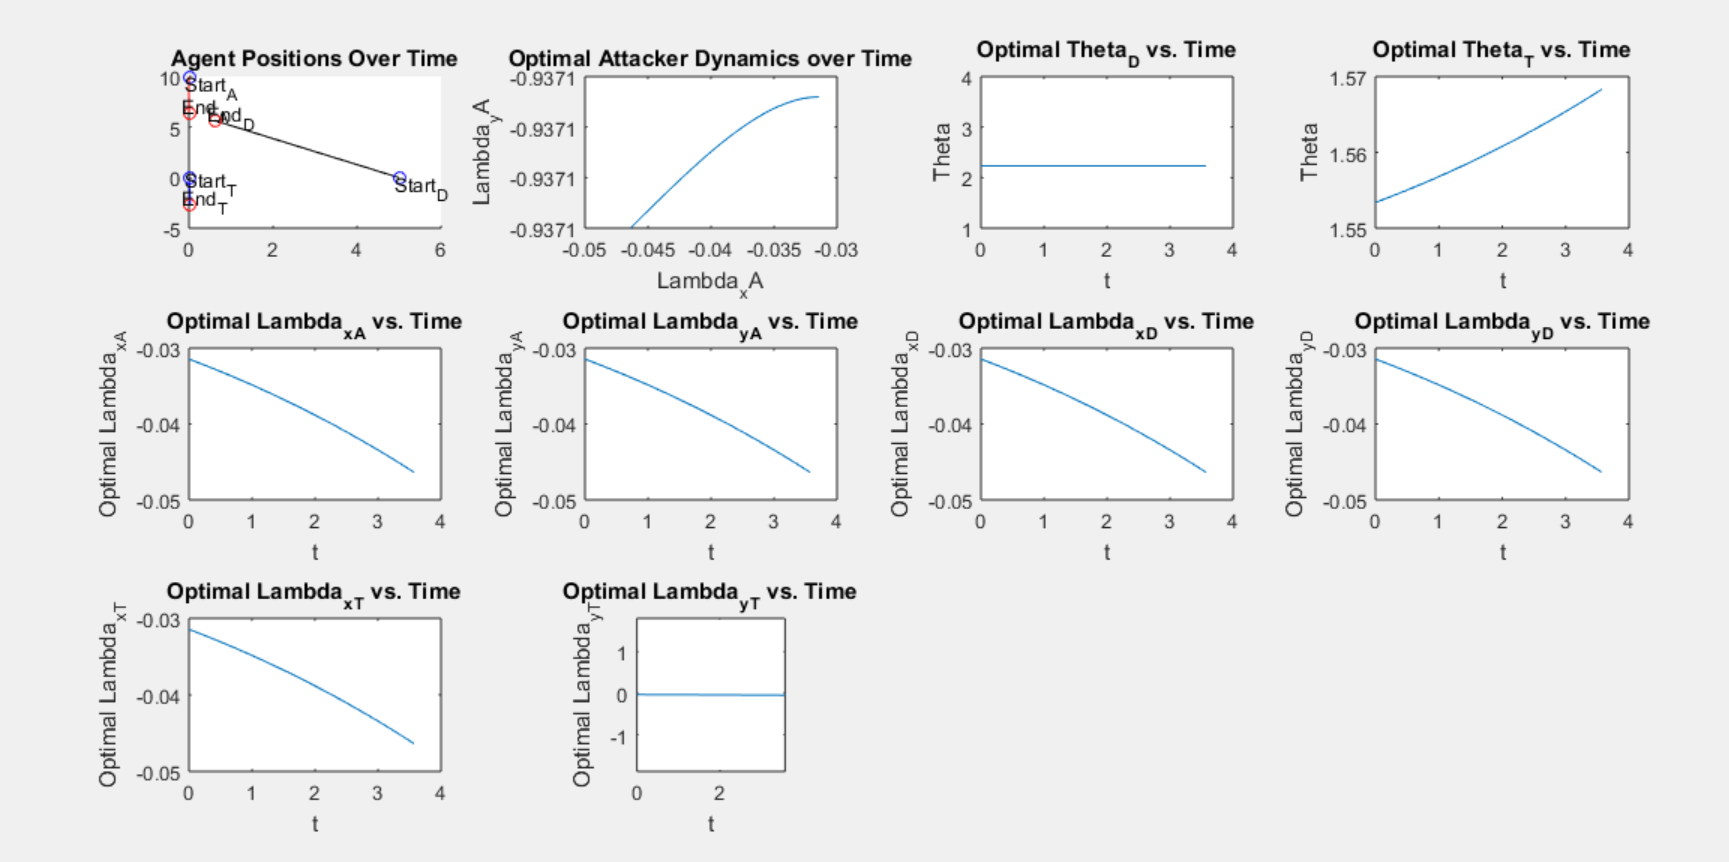
\includegraphics[width=6in]{prob3indirect.png}
\caption{Problem 3 Solved Directly}
\label{fig:prob3indirect}
\end{figure}

A zoomed-in version of the state for all agents is shown in Figure \ref{fig:prob3zoom}.


\clearpage


\begin{figure}[!h]
\centering
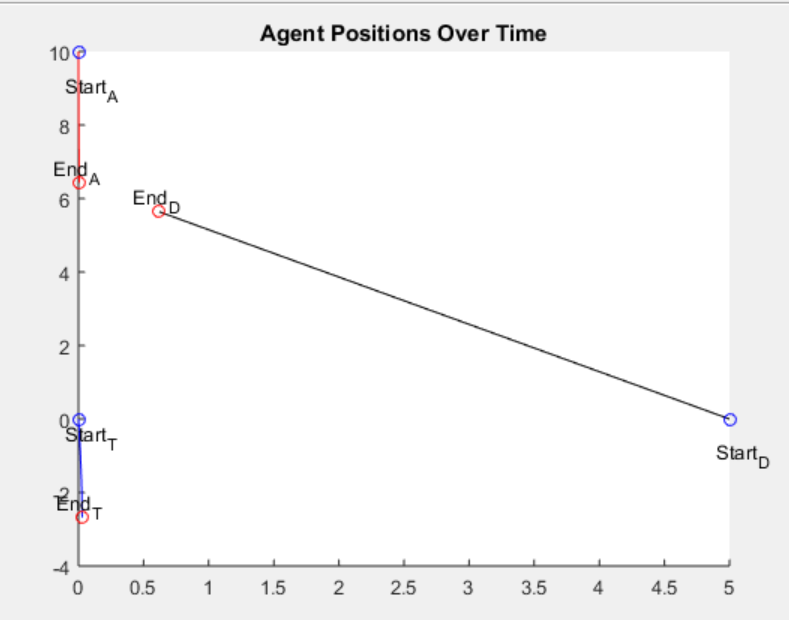
\includegraphics[width=5in]{prob3zoom.png}
\caption{Problem 3 State Expanded}
\label{fig:prob3zoom}
\end{figure}

As can be seen, the answer ended up being the same as when a new $\theta_A$ was used. The answers with $\theta_A$ were deleted long ago, unfortunately. 

The answer is actually slightly different in that the target does not seem to travel exactly straight. This is likely due to some error in terminal conditions, however, it is easily inferred that traveling straight down would be more optimal.

Problem 3 was not solved via direct shooting, however, it would have been attempted in the same manner as the other problems (with a general form of the dynamics known).


\section*{Problem 4}

Problem 4 was solved via direct shooting in the file \path{problem4Direct.m}, which depends on \path{directUtility.m}, \path{directDynamics.m}, and \path{directConstraint.m}.

The formulas derived analytically are attached. In the end, we find at $t_0$:

\begin{equation}
\begin{aligned}
\label{eq:2}
x(t_0) &= 0 \\
y(t_0) &= 1 \\
\lambda_x(t_0) &= ? \\
\lambda_y(t_0) &= ? \\
\end{aligned}
\end{equation}

And at $t_f$:

\begin{equation}
\begin{aligned}
\label{eq:2}
x(t_f) &= 10 \\
y(t_f) &= 1 \\
\lambda_x(t_f) &= ? \\
\lambda_y(t_f) &= ? 
\end{aligned}
\end{equation}

Leaving the final values to solve for as $t_f$, $x(t_f)$, $\lambda_x(t_f)$, $\lambda_y(t_f)$, $\lambda_x(t_0)$ and $\lambda_y(t_0)$.

For the direct shooting dynamics we can again guess the general form. The same equations as in problem 1 were used. After performing direct shooting, the solution in Figure \ref{fig:prob4direct} was found.


\clearpage


\begin{figure}[!h]
\centering
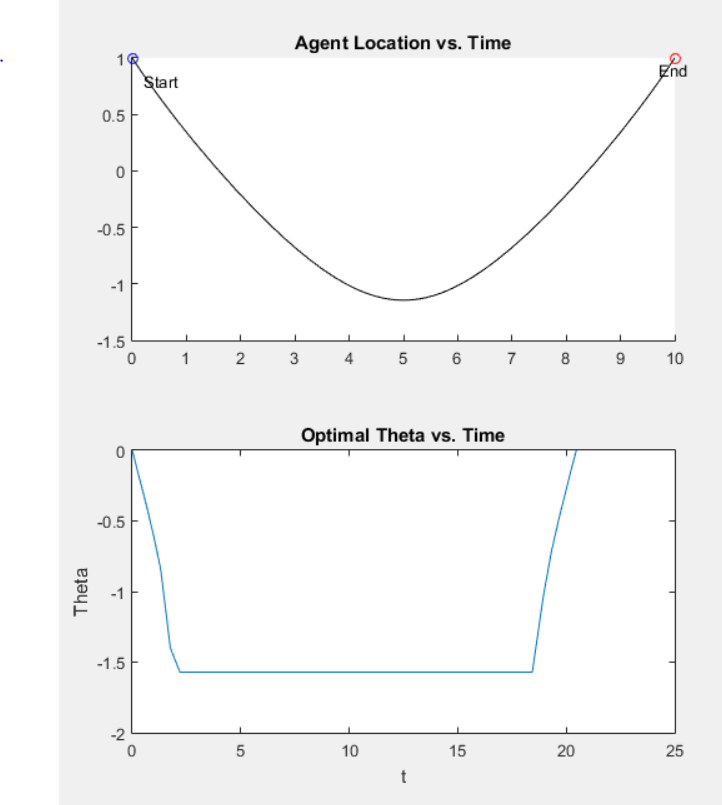
\includegraphics[width=4in]{prob4direct.png}
\caption{Problem 4 Solved Directly}
\label{fig:prob4direct}
\end{figure}

We again experience the same issue of not having a way to directly see theta, and have to find it with inverse sin. The solution.

Because of the high number of unknowns in the problem and the knowledge of the form of the dynamics, direct shooting is a great choice. Indirect backwards shooting was also attempted. using \path{problem4.m}, which depends on \path{dynamics4.m}, \path{error4_backwards.m}, and \path{error4_backwards.m}. After performing backwards shooting, the solution in Figure \ref{fig:prob4indirect} was found.

\begin{figure}[!h]
\centering
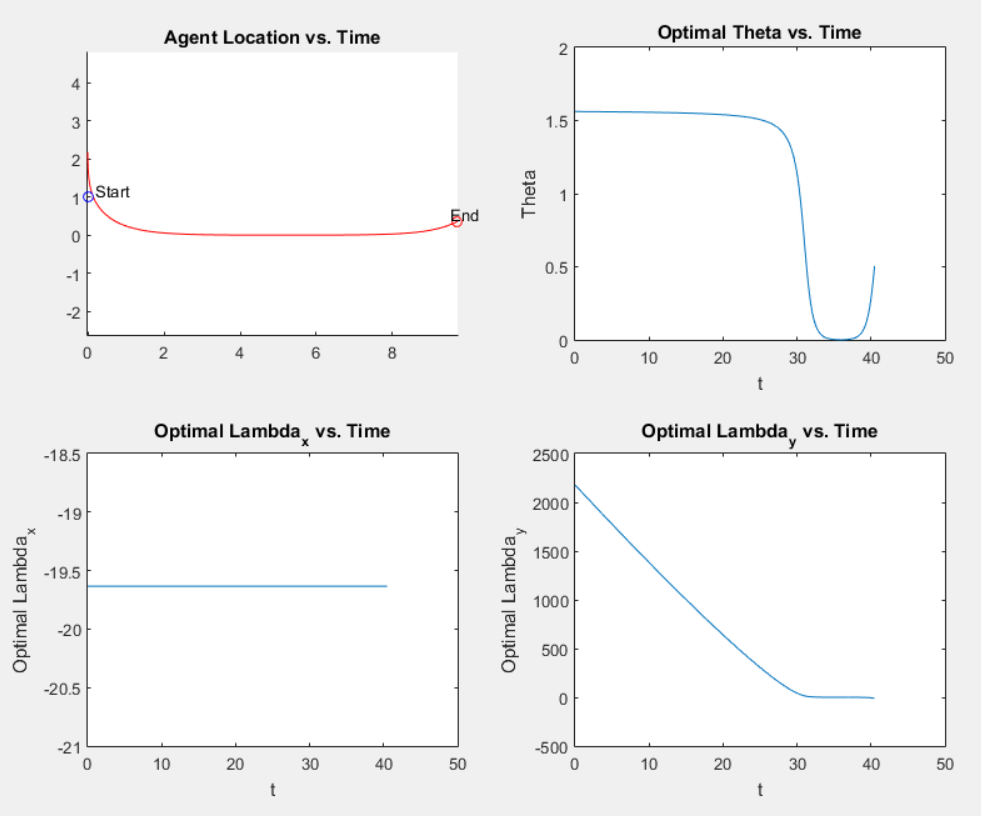
\includegraphics[width=5in]{prob4indirect.png}
\caption{Problem 4 Solved Indirectly}
\label{fig:prob4indirect}
\end{figure}

Figure \ref{fig:prob4indirect} shows difficulty in finding an indirect solution that matched the direct solution. Many different guesses were attempted, especially ones based on the found direct solution, but they were unsuccessful. 



\clearpage


Problem 4, unlike the other problems, was found to be easier to solve with direct shooting than with indirect shooting. This is likely due to the complex adjoint dynamics and high number of unknowns in comparison to other problems. It is also inconvenient once again that theta is unable to be recovered, though using dynamics in terms of lambdas yielded the best final results.

\iffalse
\section*{Problem 1}
Answer to the problem goes here.

\begin{enumerate}
  \item
   Problem 1 part 1 answer here.
  \item
    Problem 1 part 2 answer here.

    Here is an example typesetting mathematics in \LaTeX
\begin{equation*}
    X(m,n) = \left\{\begin{array}{lr}
        x(n), & \text{for } 0\leq n\leq 1\\
        \frac{x(n-1)}{2}, & \text{for } 0\leq n\leq 1\\
        \log_2 \left\lceil n \right\rceil \qquad & \text{for } 0\leq n\leq 1
        \end{array}\right\} = xy
\end{equation*}

    \item Problem 1 part 3 answer here.

    Here is an example of how you can typeset algorithms.
    There are many packages to do this in \LaTeX.
     
    \lstset{caption={Caption for code}}
    \lstset{label={lst:alg1}}
     \begin{lstlisting}[style = Python]
    from package import Class # Mesh required for..
    
    cinstance = Class.from_obj('class.obj')
    cinstance.go()
    \end{lstlisting}
     
  \item Problem 1 part 4 answer here.

    Here is an example of how you can insert a figure.
    \begin{figure}[!h]
    \centering
    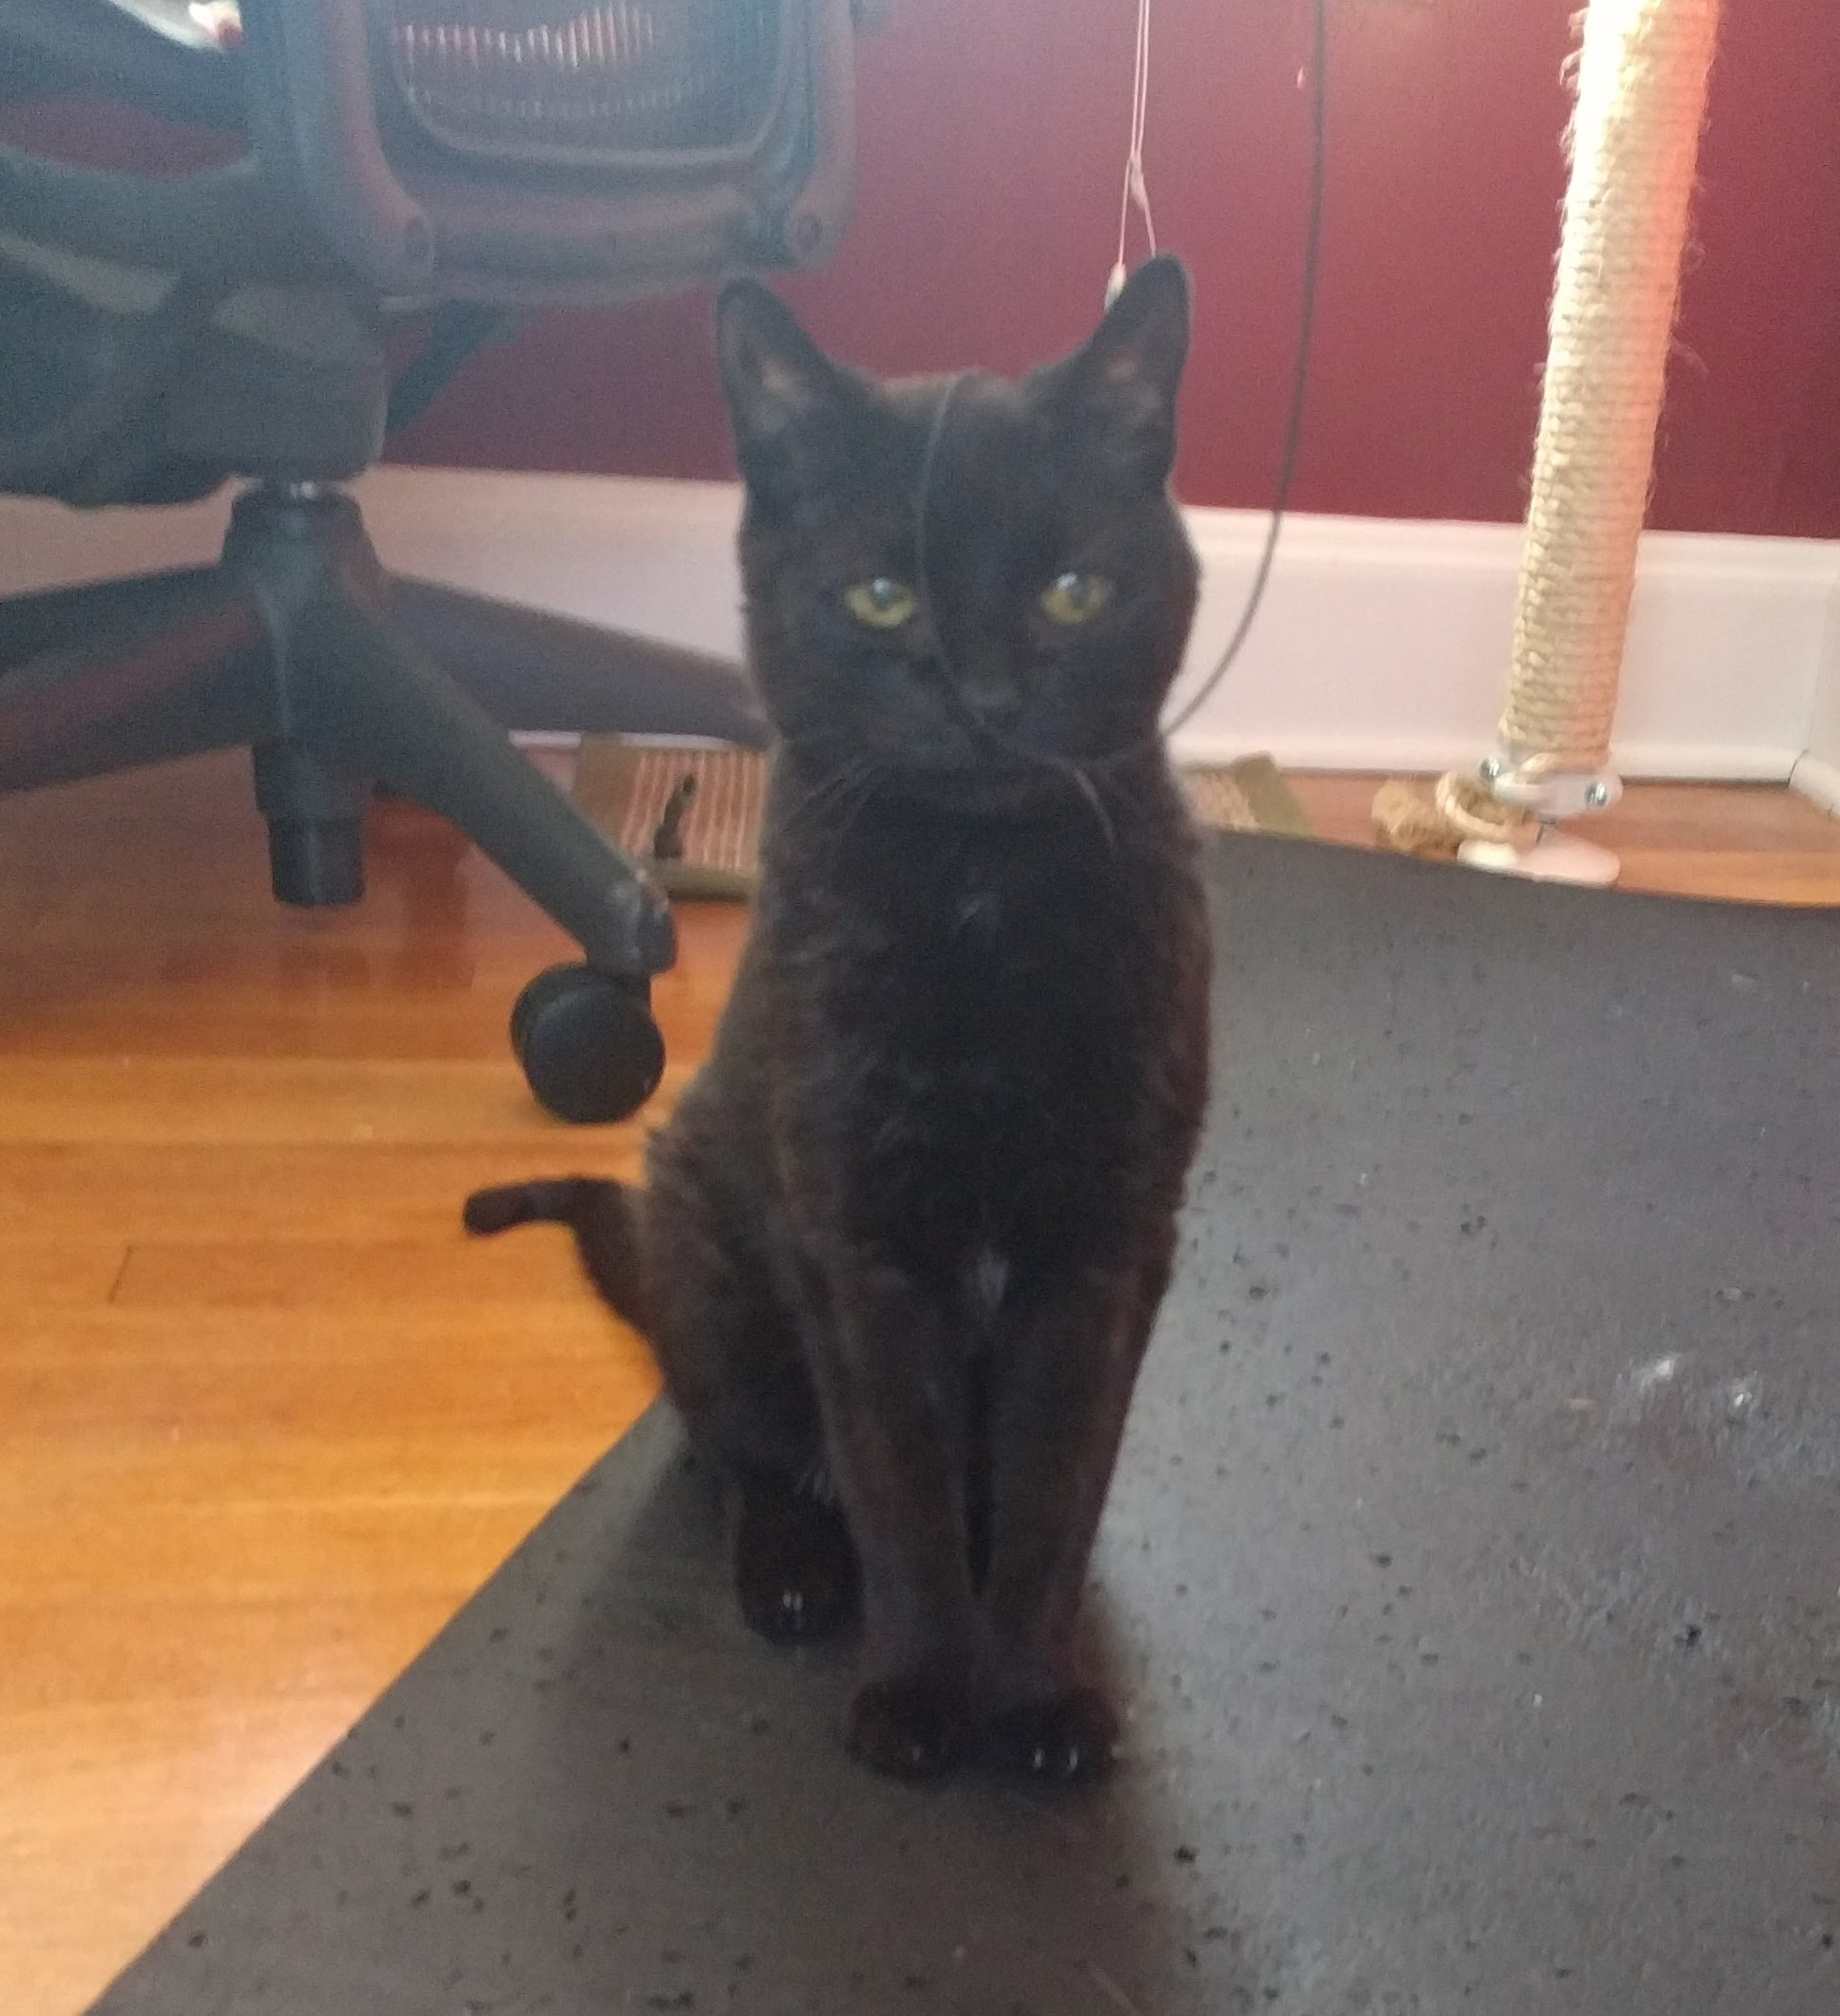
\includegraphics[width=0.3\linewidth]{heidi.jpg}
    \caption{Heidi attacked by a string.}
    \end{figure}
\end{enumerate}


\section*{Problem 2}
% Rest of the work...

\fi

\end{document}
